% !TEX root = rapport.tex
\section{History}
\label{history}
In 1946, the ENIAC computer was completed for the United States Army and it has been argued whether ENIAC is to be seen as the first digital computer\cite{McCartney1999}, or if this title actually belongs to the ABC\cite{court} computer (1942). Regardless, the history of the underlying computer interfaces used is longer than the history of computers themselves.

Already in the beginning of the 18th century Basile Bouchon started using perforated paper to control the textile looms used for weaving. To control the cords of a warp, thick paper rolls were punched with patterns of holes, each column corresponding to a cord. The cords were then raised or lowered, depending on whether the paper was punched or not. In this manner Bouchons machine managed to automatise part of the weaving process, and allowed for more complex weaving patterns. Although punched cards were first invented in the 18th century, they were used as means of interaction both by the ABC and the ENIAC right at the beginning of modern computer history, and they saw continued use until the late 1980's \cite{aspray1990ch4}.

\begin{figure}[h!]
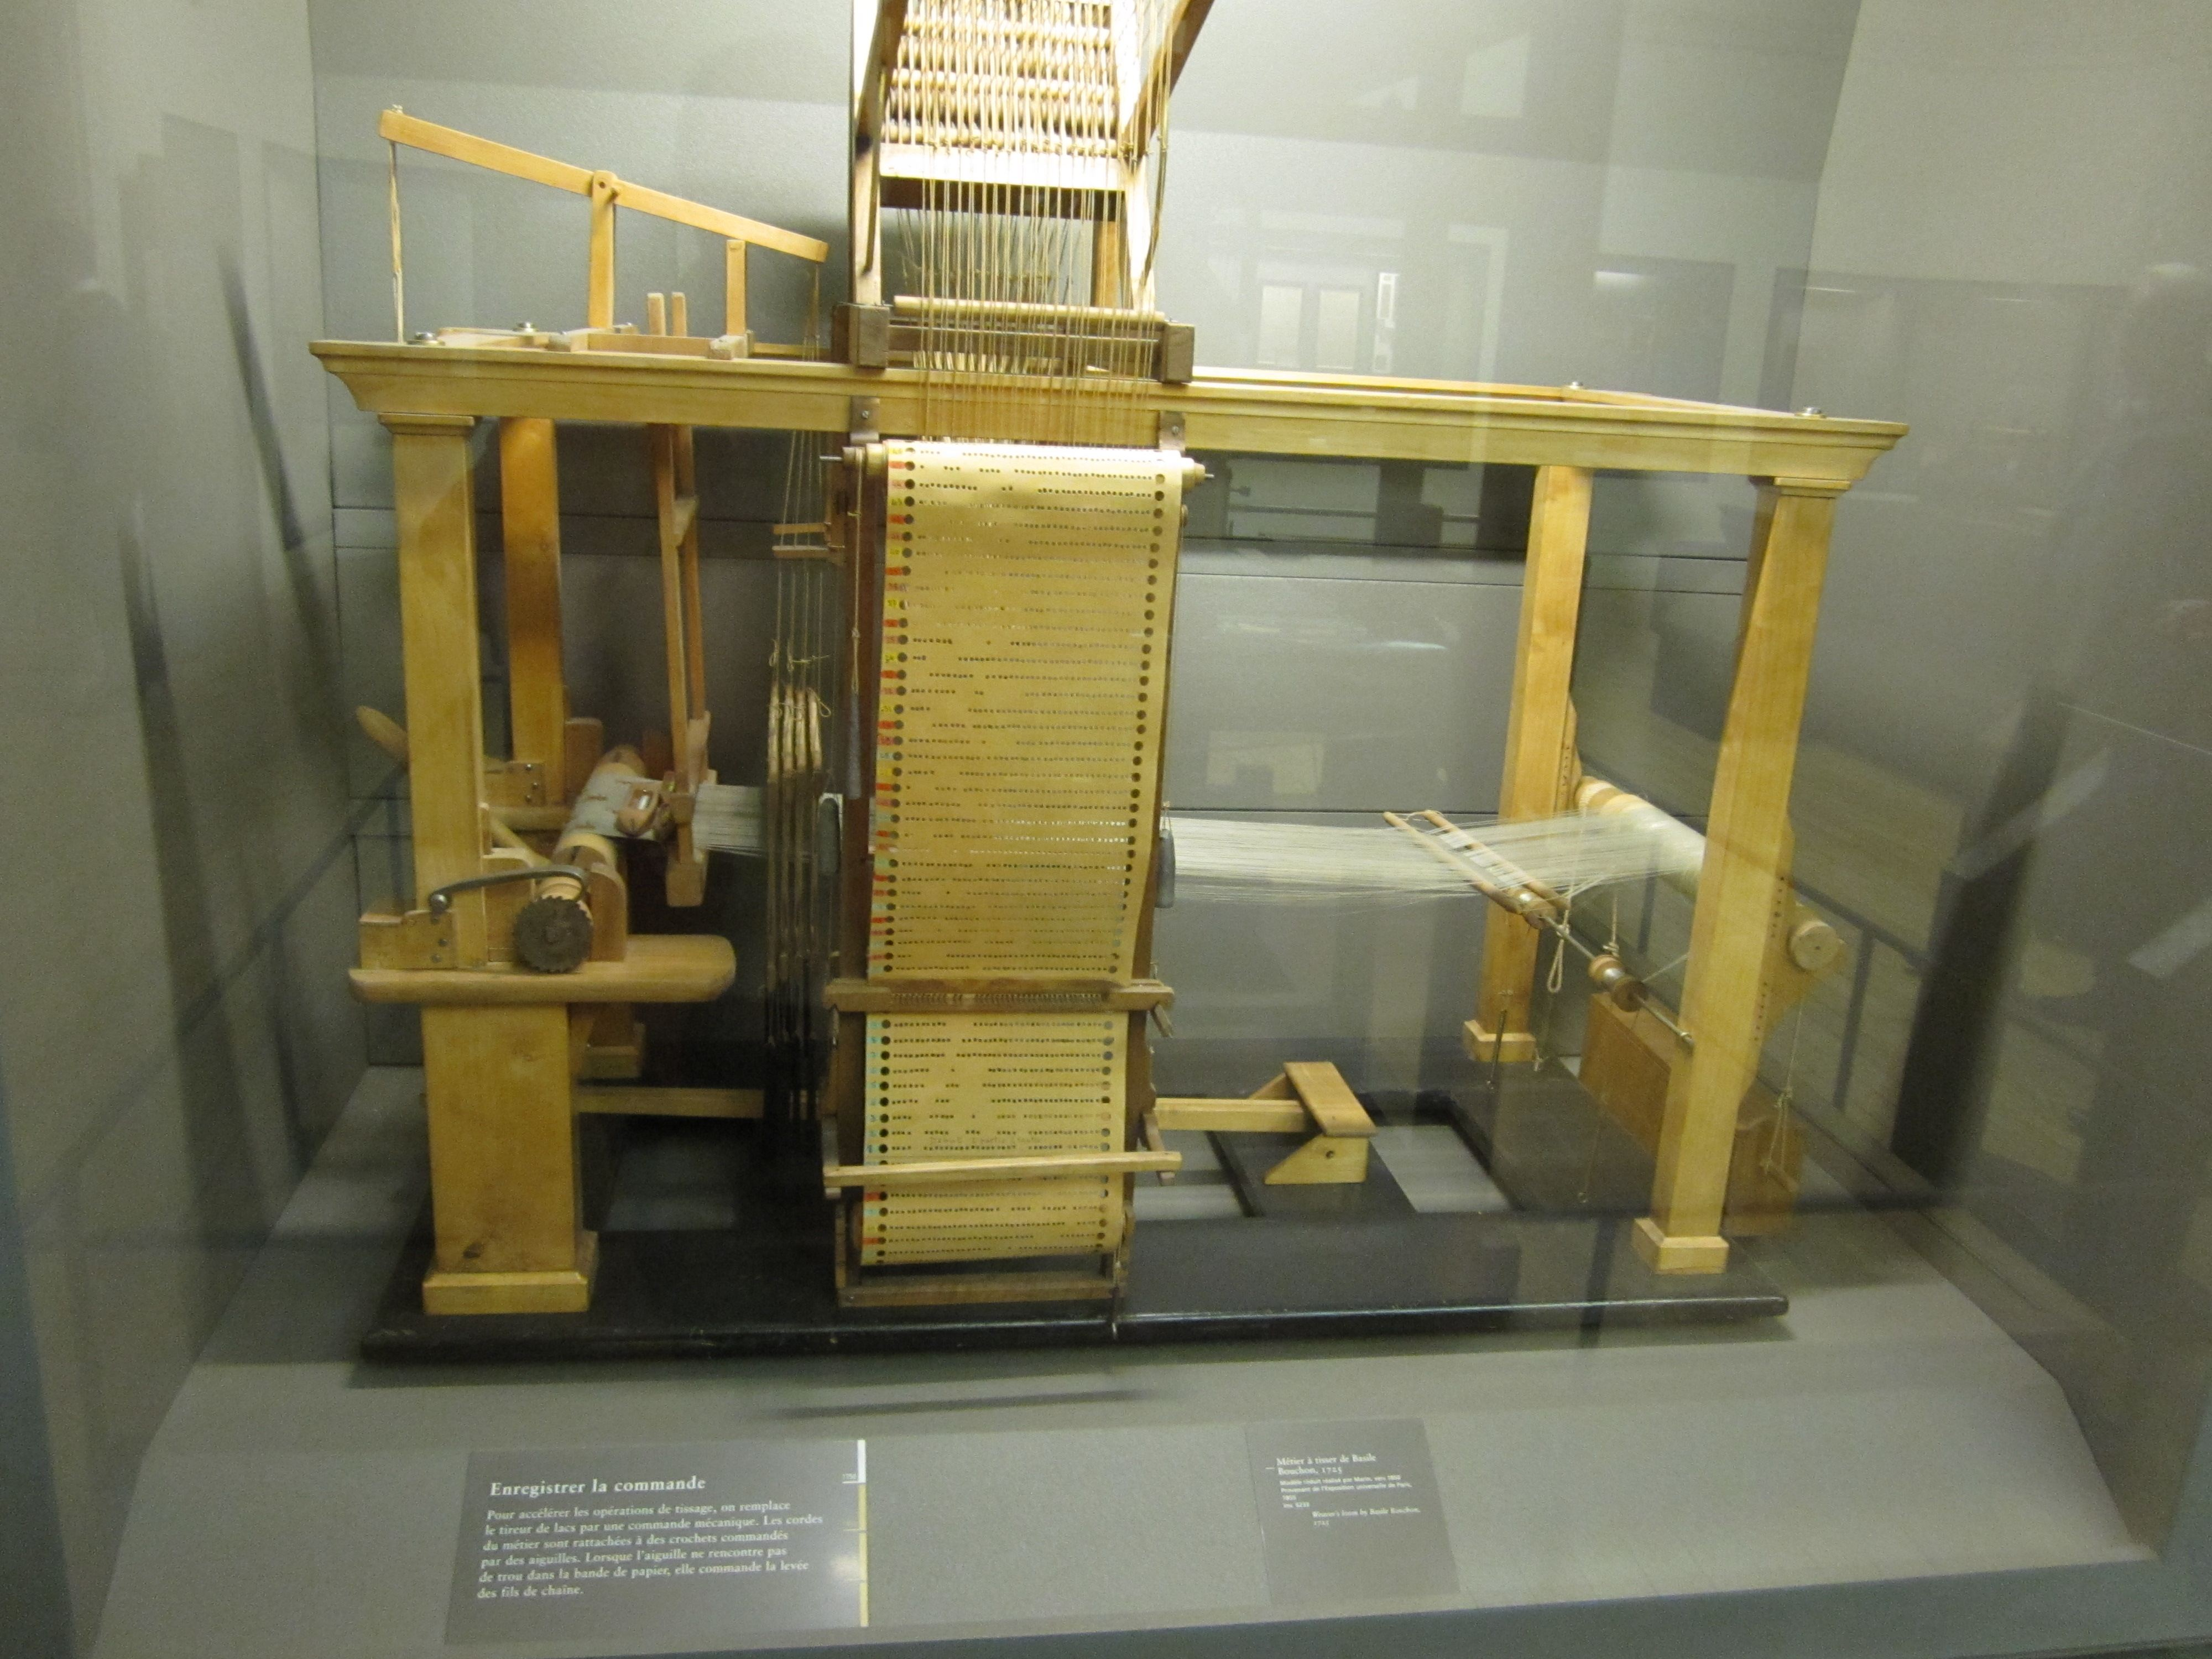
\includegraphics[width=0.8\textwidth] {bilder/bouchonloom.jpg}
\caption{A Bouchon loom exhibited at the Musée des arts et métiers in Paris.}
\end{figure}
% Bild på bouchon loom
\nocite{bouchonloom}


\subsection{Herman Hollerith and the Census Problem}
By the end of the 19th century, the Bureau of the Census in the United States had a problem. The Census is the agency in charge of keeping records of the population, and due to heavy immigration, the amount of data and complexity of the system was rapidly increasing. At that time, the Census was performing a population count every ten years - a process taking several years to complete. In 1889, the director of the Census advertised a competition for the 1890 census tabulation system. The winner of the competition was Herman Hollerith, a former employee of the census bureau, with his electric tabulating machine.\cite{aspray1990ch4}

\begin{figure}[h!]
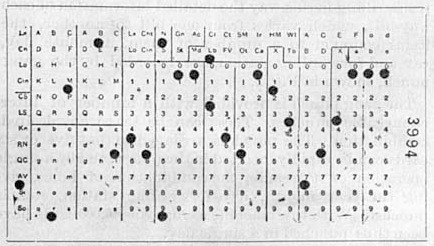
\includegraphics[width=0.8\textwidth] {bilder/punchedcard.jpg}
\caption{A punched card used in the 1890 Census, published in the Railroad Gazette 1895.}
\end{figure}
% Bild på punched card
\nocite{punchcard}

Hollerith's tabulating machine was a success, and the contract was renewed for the 1900 census. In order to expand the customer base of his tabulating machines, Hollerith founded the Tabulating Machine Company in 1896. His company was one of three companies that in 1911 merged to form the Computing Tabulating Recording Company (CTR) - later renamed IBM\cite{IBMhistory}.

Punched cards were the most commonly used data medium until the 1950s, and were commonly used until the mid 1980s when they had become obsolete by the \emph{computer terminal}\cite{aspray1990ch4}.

\subsection{The Teleprinter and the Terminal}
In 1901, Donald Murray developed a \emph{tele-typewriter} or \emph{teleprinter}. His idea was to simplify the work of telegraph operators, by using a typewriter keyboard. The operator would type on a typewriter, where every letter corresponded to a pattern of holes punched into a punch card. The information on the punch card was then transfered over the already existing telegraph lines and reproduced at the receiving end, again on punch cards\cite{page1901world}.

This method of typing to punch cards was used by early computers, and are known as \emph{computer terminals} but the term computer terminal is not exclusive to punch card-based typewriters. Though punch cards were the main method of data entry and data storage, alternative methods began to emerge in the early 1960's. 

In the 1960's, output devices had become more advanced and in the end of the 1960's, the first attempts were made to replace printing with a \emph{computer monitor}. This method of combining a typewriter-style \emph{keyboard} with a monitor is what constitutes a computer terminal. One of the earliest computer terminals was the Datapoint 3300 by the Computer Terminal Corporation\cite{datapoint}. Using the Datapoint 3300, the user could control a \emph{cursor} by moving it up, down, left and right on the screen.

Later computers with microprocessors allowed program and working memory to be shared and for computer programs to read data from the memory itself. To input data into the memory, punch cards could still be used. However, since all the data was stored electronically the data could as well be entered direcly into the memory. This removed the need for punched paper to be used as a middle step. The data previously transmitted via telegraph lines could be used to connect the typewriter directly to the computer memory. The initial disadvantage with this method was that memory was limited and expensive. Thus, the use of punch cards declined in favour of the computer terminal, in step with computer displays becoming more available\cite{aspray1990ch4}.

\subsection{Pointing devices}
The first computer \emph{mouse} was developed in 1965 at the Stanford Research Laboratory and is attributed to Doug Engelbart. Engelbart also proposed applications for the mouse, such as using multiple tiled \emph{windows}, which became widely used in early graphical computer interfaces. Although invented in the 1960's, it was not commercially available until 1981 when released as part of the Xerox Star system\cite{myers1998bhh}. Xerox soon got competition by the Apple Lisa (1983) and the popular Apple Macintosh (1984).

\begin{figure}[h!]
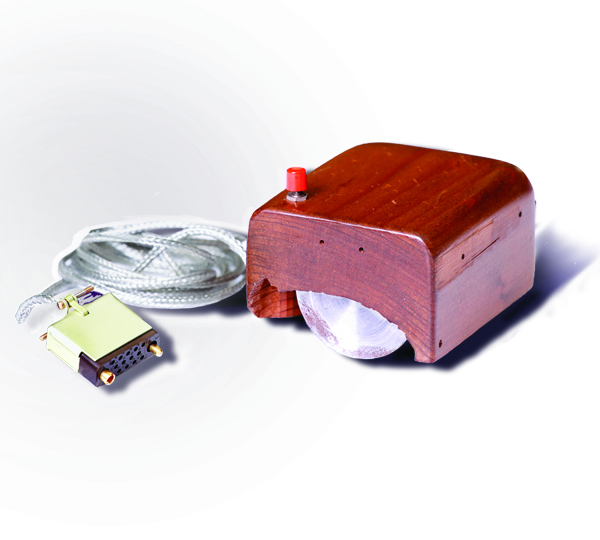
\includegraphics[width=0.8\textwidth] {bilder/firstmouse.jpg}
\caption{The first mouse prototype by Engelbart 1865.}
\end{figure}
% Bild på första musen
\nocite{srimouse}

\begin{figure}[h!]
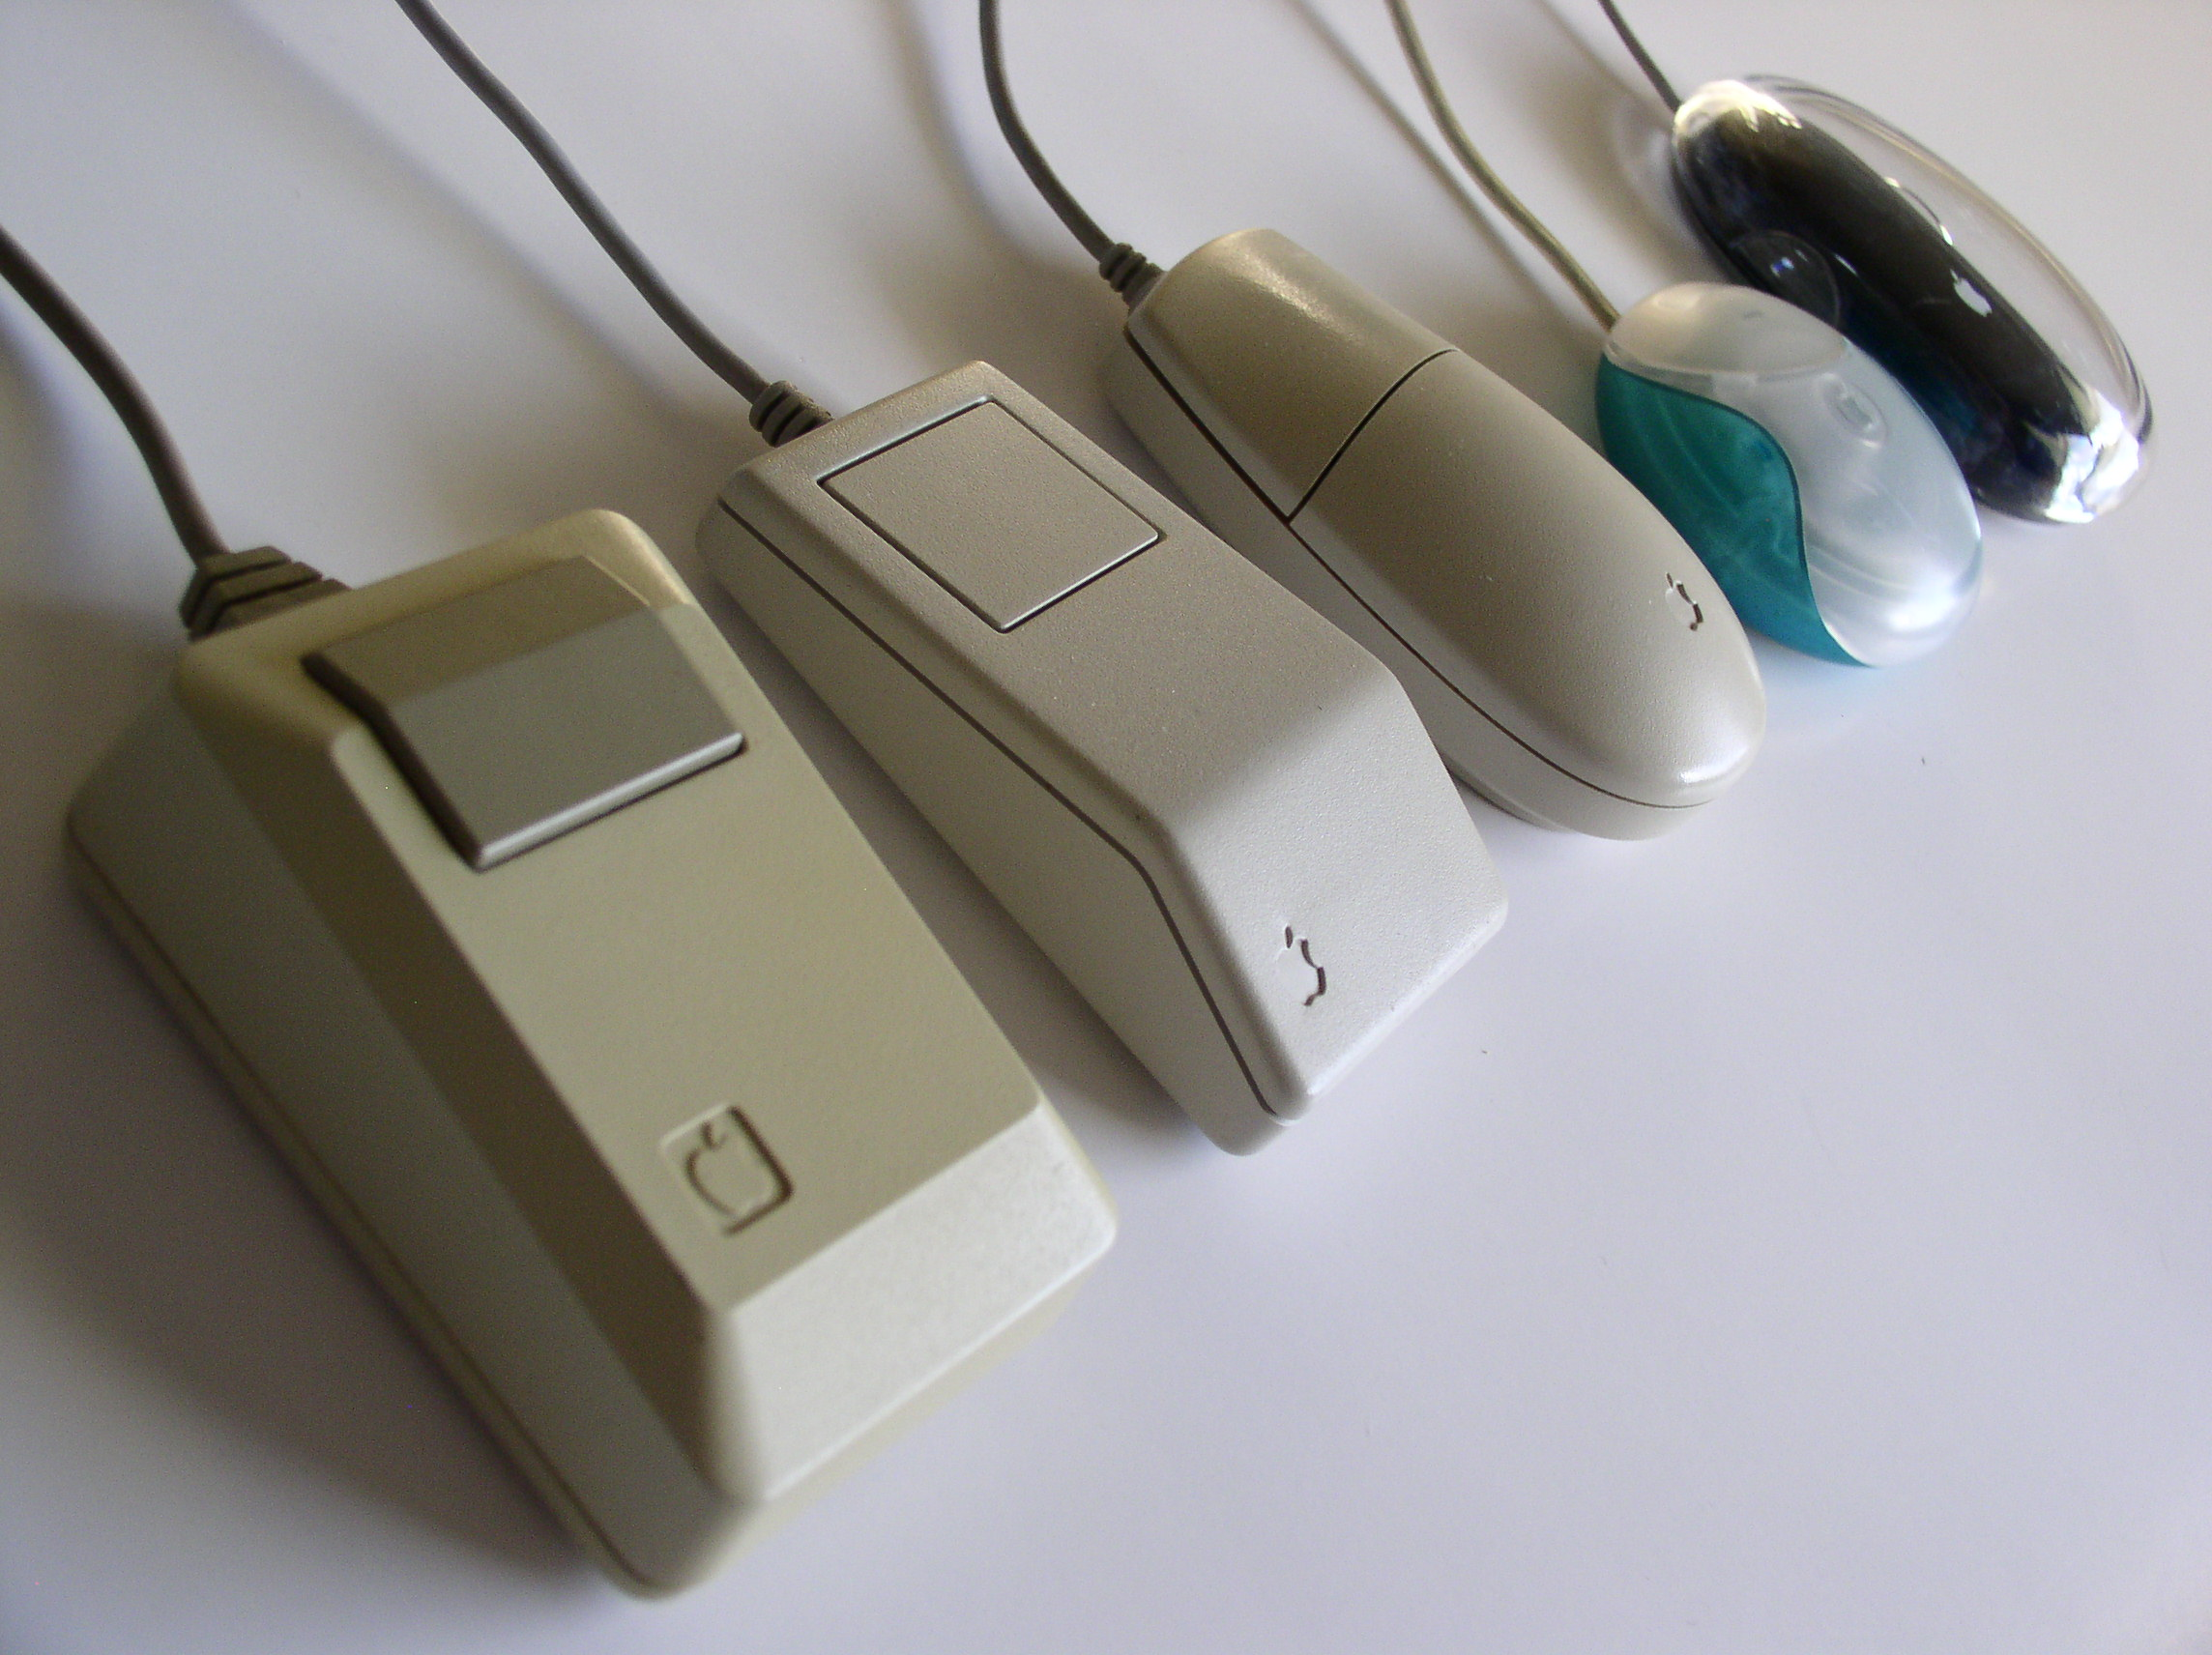
\includegraphics[width=0.8\textwidth] {bilder/applemice.jpg}
\caption{A series of mice from the Apple company from different era. The first Apple Macintosh was supplied with the Macintosh mouse (closest in the picture).}
\end{figure}
% Bild på xerox-musen eller mac-musen
\nocite{applemice}

The introduction of the mouse allowed the users to move a pointer on the display that could be used to interact with the computer. A ball underneath the mouse gave relative Cartesian coordinates when rolling the ball on a surface.

The mouse laid the ground for the WIMP (Windows, Icon, Menus, Pointer) graphical interfaces used today\cite{journals/cacm/Dam97}. The graphical user interface was invented by XEROX, and the Star system is wildely recognised as the first commercially available product with a graphical interface. 

As the displays became smaller and smaller and with the introduction of flat screens the portable computers were introduced. To keep these computers portable the mouse had to be built into the computer itself. This lead to a different kind of pointing devices, which are described in the following section. 

